\documentclass[11pt,a4paper]{article}

% Packages used
\usepackage[utf8]{inputenc}
\usepackage{amsmath, amssymb, amsbsy, amsthm}
\usepackage{enumerate} % To enumerate with roman numbers
\usepackage{makeidx}
\usepackage{graphicx}
\usepackage{color}
\usepackage[usenames,dvipsnames]{xcolor}
\usepackage[hidelinks]{hyperref}
\usepackage{xspace}
\usepackage{dsfont}
\usepackage{marvosym}
\usepackage{array}
\usepackage[width=16.00cm, height=27.00cm]{geometry}
\usepackage{relsize} % \mathlarger
\usepackage{algpseudocode} % Algorithms
\usepackage{algorithm} % Algorithms
\usepackage{colortbl}

\setlength{\parindent}{0pt} % To avoid margins.

\title{Forecasting the Minimum Cost of Monthly Survival During\\the Syrian Civil War}
\author{Aneesh Dahiya${}^\ast$, Jaco Fuchs${}^\ast$, Christoph Glanzer${}^\ast$, Julia Ortheden\thanks{Authors are listed in alphabetical order as they contributed equally.}}
\date{}

\parindent=0pt % To avoid margins

% %%%%%%%%%%%%%% %
% Extra Commands %
% %%%%%%%%%%%%%% %

\newcommand{\Z}{\mathbb{Z}}
\newcommand{\R}{\mathbb{R}}
\newcommand{\Q}{\mathbb{Q}}
\newcommand{\N}{\mathbb{N}}
\newcommand{\inv}{^{-1}}
\newcommand{\invtransp}{^{-T}}
\newcommand{\spann}{\text{span}}
\newcommand{\lattice}{\mathcal{L}}
\newcommand{\hnf}{\texttt{HNF}\xspace}
\newcommand{\tu}{\texttt{TU}\xspace}
\def\T{^\mathrm{T}}
\newcommand{\argmin}{\, \mathrm{argmin} \,}
\newcommand{\argminn}[2]{\mathrm{arg} \, \underset{#1}{\mathrm{min}} ~ #2}
\newcommand{\argmax}{\, \mathrm{argmax} \,}
\newcommand{\argmaxx}[2]{\mathrm{arg} \, \underset{#1}{\mathrm{max}} ~ #2}
\newcommand{\latticei}[1]{\lattice_{#1}^*}
\newcommand{\supp}[1]{\mathrm{supp} \left( #1 \right)}
\newcommand{\rank}{\mathrm{rank}}
\newcommand{\sublattice}[1]{\lattice_{#1}}
\newcommand{\mo}[1]{\, \mathrm{mod} \, 1}
\renewcommand{\mod}[2]{#1 \, \mathrm{mod} \, #2}
\newcommand{\ip}{\texttt{IP}\xspace}
\newcommand{\ips}{\texttt{IP}s\xspace}
\newcommand{\lp}{\texttt{LP}\xspace}
\newcommand{\lps}{\texttt{LP}s\xspace}
\newcommand{\norm}[1]{\left\lVert#1\right\rVert}
\newcommand{\abs}[1]{\left|#1\right|}
\newcommand{\vtcs}{\texttt{V}\xspace}
\newcommand{\arcs}{\texttt{A}\xspace}
\newcommand{\edges}{\texttt{E}\xspace}
\newcommand{\dprime}{{\prime\prime}}
\newcommand{\quotmarks}[1]{``#1''}
\newcommand{\nth}[2]{\ensuremath{{#1}^{\text{\tiny{#2}}}}\xspace}
\newcommand{\detmax}{\vartriangle}
\newcommand{\inc}[1]{\chi^{#1}}

\def\conv{\operatorname{conv}}
\def\aff{\operatorname{aff}}
\def\st{\operatorname{ s.t. }}
\def\lin{\operatorname{lin}}
\def\dom{\operatorname{dom}}
\def\int{\operatorname{int}}
\def\relint{\operatorname{relint}}
\def\rec{\operatorname{rec}}

\def\cone{\operatorname{cone}}
\def\vol{\operatorname{vol}}

% Amsmath
\newtheorem{definition}{Definition}
\newtheorem{lemma}[definition]{Lemma}
\newtheorem{theorem}[definition]{Theorem}
\newtheorem{corollary}[definition]{Corollary}
\newtheorem{remark}[definition]{Remark}
\newtheorem{notation}[definition]{Notation}
\newtheorem{note}[definition]{Note}

% Renewing commands for Algorithmic
\renewcommand{\algorithmicrequire}{\textbf{Input:}}
\renewcommand{\algorithmicensure}{\textbf{Output:}}
\algtext*{EndIf} % Remove "end if" text
\algtext*{EndFor} % Remove "end for" text
\algtext*{EndWhile} % Remove "end while" text

% Change enumeration sign
%\def\labelitemi{\tiny$\blacksquare$}
\def\labelitemi{\raisebox{1pt}{\scalebox{0.45}{$\blacksquare$}}}

% Extend matrix size
\setcounter{MaxMatrixCols}{20}

% Polyhedron-Environment
\makeatletter
\newenvironment{constraints}{\let\scriptstyle\textstyle\begin{subarray}{l}} {\end{subarray}}
\makeatother

% %%%%%%%%%%%%% %
% Main Document %
% %%%%%%%%%%%%% %

\begin{document}
	\maketitle
	
	\section*{Motivation and Summary}
	It is becoming more and more of a common practice for aid organizations and NGOs to deliver cash-based assistance to war-town countries such as Syria. On average, it takes three to six weeks to deliver aid to the local population. It is therefore crucial to forecast the minimum cost of monthly survival (SMEB, "survival minimum expenditure basket") to ensure that the aid delivered is neither too high nor too low. The goal of this project is to develop a model to forecast the SMEB price. 
	
	When predicting a single month into the future, the baseline model which simply uses the value from the previous month as a prediction for the next month outperforms all of the models which we have tested. We believe that this is due to the high volatility of the SMEB price. For a forecast of two or more months into the future, we present a variant of an \texttt{ARIMA} model which outperforms the baseline model.\\
	
	This project is joint work with IMPACT Initiatives as part of the "Hack4Good" project of the Analytics Club at ETH Zürich.
	
	\section*{Structure of the Data}
	A file in the .xlsx format containing the monthly price development of various products in all governorates, districts and subdistricts from February 2017 to August 2019 is provided. Unfortunately, around 60\% of the data is missing.
	
	From this data the SMEB prices in Syrian Pounds are extracted on all available levels of regional granularity. The decision to use the SMEB price in Syrian pounds was taken together with the other teams since the currency exchange rate between the local currency and USD does not have to be taken into account.
	
	To handle the missing data, we use the following quick-fix: If a missing data point lies in between given data, linear interpolation is used and otherwise, the data point is excluded. We have chosen this simple approach as a different team was given the task of finding more sophisticated approaches towards solving the imputation problem.
	
	\section*{Model Exploration}
	We have focused on implementing three types of models to generate predictions for future SMEB prices: Linear (auto-)regression, time-series based models and neural networks. In order to compare models with each other we have used a simple common evaluation metric based on a time-series adapted cross validation procedure: A model is trained on all datapoints up to February 2018. Then, the next month (March 2018) is predicted. Next, the model is retrained on all previous datapoints, including the true value of March 2018, and once again the next month (April 2018) is predicted. This procedure is repeated consecutively. Finally, the relative mean squared error between all predicted and true values is calculated and averaged. Table \ref{fig:numbers} shows a quick overview for the district level.\footnote{We want to emphasize that these values were generated using the SMEB prices without water as this data is subject to a lesser number of missing values. In the code provided, we use the SMEB prices with water in Syrian pounds, which is why the results may differ.}
	
	\begin{table}
		\centering
		\begin{tabular}{|l|l|}
			\cline{1-2}
			Model & Rel. MSE \\ \cline{1-2}
			~ & ~ \\[-4.6mm]
			\rowcolor{green} Baseline Model & 1,79 \\
			\rowcolor{red} Linear Momentum & 4,34 \\
			\rowcolor{red} Savitzky-Golay extrapolation & 3,67 \\
			\rowcolor{red} ElasticNetCV & 5,97 \\
			\rowcolor{red} RANSACRegressor & 6,01 \\
			\rowcolor{red} \texttt{LOESS}+\texttt{ARMA(p,q)} & 3,34 \\
			\rowcolor{orange} Lasso & 2,66 \\
			\rowcolor{orange} RidgeCV & 2,87 \\
			\rowcolor{yellow} Local \texttt{LOESS} + \texttt{ARMA(p,q)} & 2,65 \\
			\rowcolor{yellow} Holt-Winters & 2,07 \\
			\cline{1-2}
		\end{tabular}
		\caption{MSE values for various models on a district level.} \label{fig:numbers}
	\end{table}
	
	\begin{figure}[h!]
		\centering
		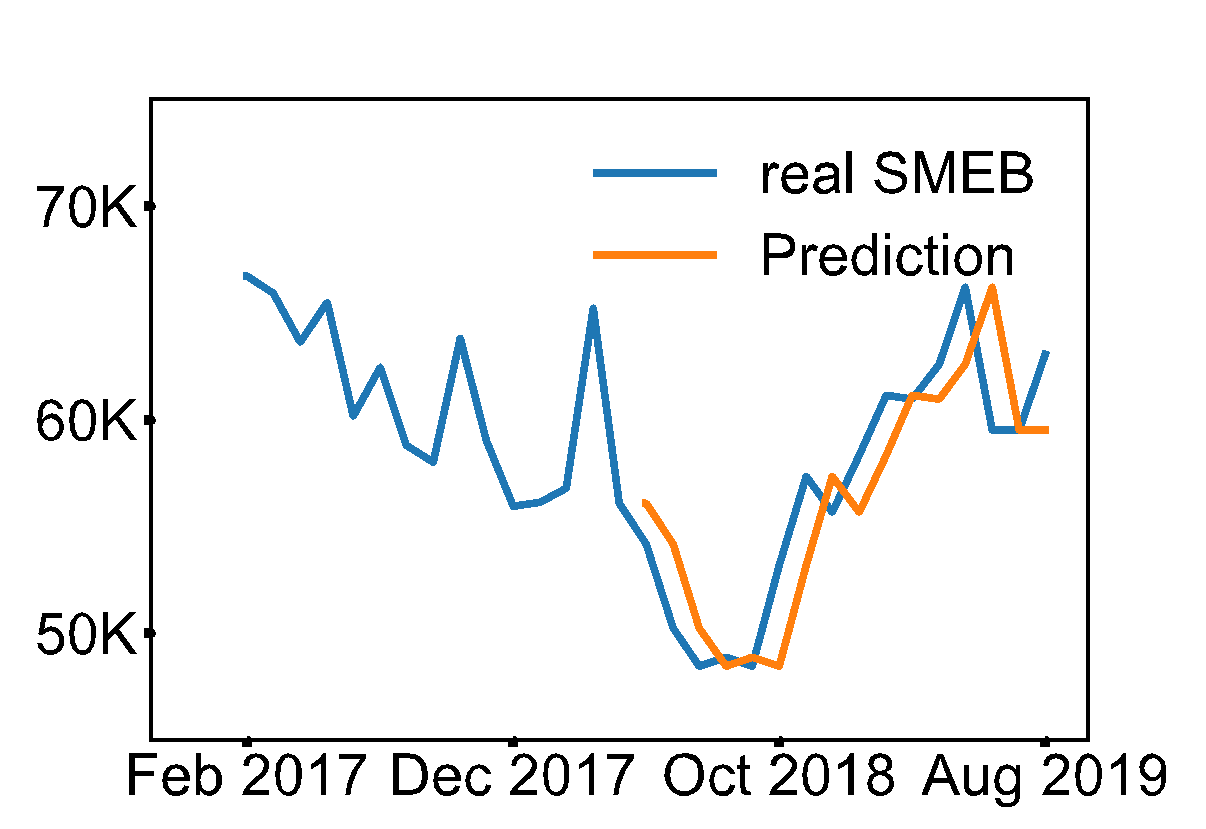
\includegraphics[width=0.5\textwidth]{image3.png}
		\caption{Due to the high volatility of the SMEB price, the baseline model serves as a good predictor for the prediction of one month into the future.}
		\label{fig:image3}
	\end{figure}

	\subsection*{Time Series Models}
	Since there was not enough data to observe seasonal effects with sufficient evidence, we fit a trend without any seasonal behavior. The models which performed best were a combination between $\mathtt{LOESS}$ (using a linear trend) and $\mathtt{ARMA}(p,q)$, and a non-seasonal Holt-Winters model. The latter, however, is a very simple exponential smoothing approach which is closely related to the baseline model.
	
	\subsection*{Linear Models}
	Regarding linear models, we have taken three different approaches.
	
	\begin{itemize}
		\item The first type of model is autoregressive and similar to \texttt{ARMA(p,q)}: When predicting the next month, the previous months are used as input features. The window length is optimized via cross validation on the time series at each instance of time. The difference between this model and \texttt{ARMA(p,q)} is that in the latter, we first fit a trend and then an autoregressive, moving average model ($\mathtt{ARMA}$) to the remainder while in the former, we assume that the time series is already a stationary process and fit an autoregressive model directly.
	
		\item The second type of linear model assumes that one of the products in the SMEB sets a \textit{trend} for the other products in the SMEB. Thus, the trendsetter's price or its last relative change is included as an additional input feature. Unfortunately, we could not identify any product as a trendsetter with sufficient evidence.
	
		\item The third type of linear model assumes that some districts are trendsetters for the SMEB price. We have identified two districts which apparently set the trend for the others, as including their SMEB price as input feature leads to a slight improvement on the common evaluation metric.
		
		To further investigate whether this is a random effect or not, we conducted the following experiment: (1) We randomly generate artificial SMEB prices. (2) We create a linear (autoregressive) model, where the "real" district data is used together with the randomly generated data as input features. (3) The model is then separately trained on all real districts as responses (one by one) using \texttt{LASSO}. (4) Subsequently, the weight which the model puts on the real features is analyzed in comparison to the weight of the artificial features. As the graph below indicates, the model seems to prefer the artificially created districts as predictors over the real district data. This implies that the observed trendsetting effect of the two districts likely comes from a random effect.
		
		\begin{figure}[h!]
			\centering
			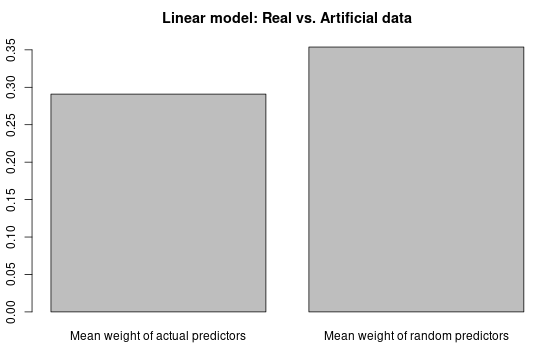
\includegraphics[width=0.66\textwidth]{image2.png}
			\caption{An experiment indicates that the predictive power of two districts as "trendsetters" which we have observed is likely a random effect.}
			\label{fig:image2}
		\end{figure}
	\end{itemize}
	
	\subsection*{Neural Networks}
	Unfortunately, most likely due to the low amount of available training points, the performance of neural network approaches was rather poor when compared to the other models.

	\section*{Predicting multiple months into the future}
	Based on our testing data, we have observed that when predicting multiple steps into the future, our \texttt{LOESS}+$\mathtt{ARMA}(p,q)$ model outperforms the baseline model.\footnote{For a prediction of $2-4$ months into the future.} As described previously, the model first fits a linear trend using the \texttt{LOESS} method. Then, an $\mathtt{ARMA}(p,q)$ model is fitted to the remainder, with an automated choice of hyper-parameters $p$ and $q$. The reason we believe that this model outperforms the baseline model for multiple steps into the future is the following: While there exists a clear trend, the price data is still highly volatile. Starting at a prediction of at least $2$ months into the future, the trend prediction kicks in and the trend becomes more significant when compared to the seemingly random volatility of the prices. Since our model uses \texttt{LOESS} to fit a trend, it performs better after a few months. However, as the trend itself changes over time, the prediction worsenes again significantly when predicting more than 4 months into the future. Figure~\ref{fig:image1} shows a prediction of 4 months into the future.
	
	\begin{figure}[h!]
		\centering
		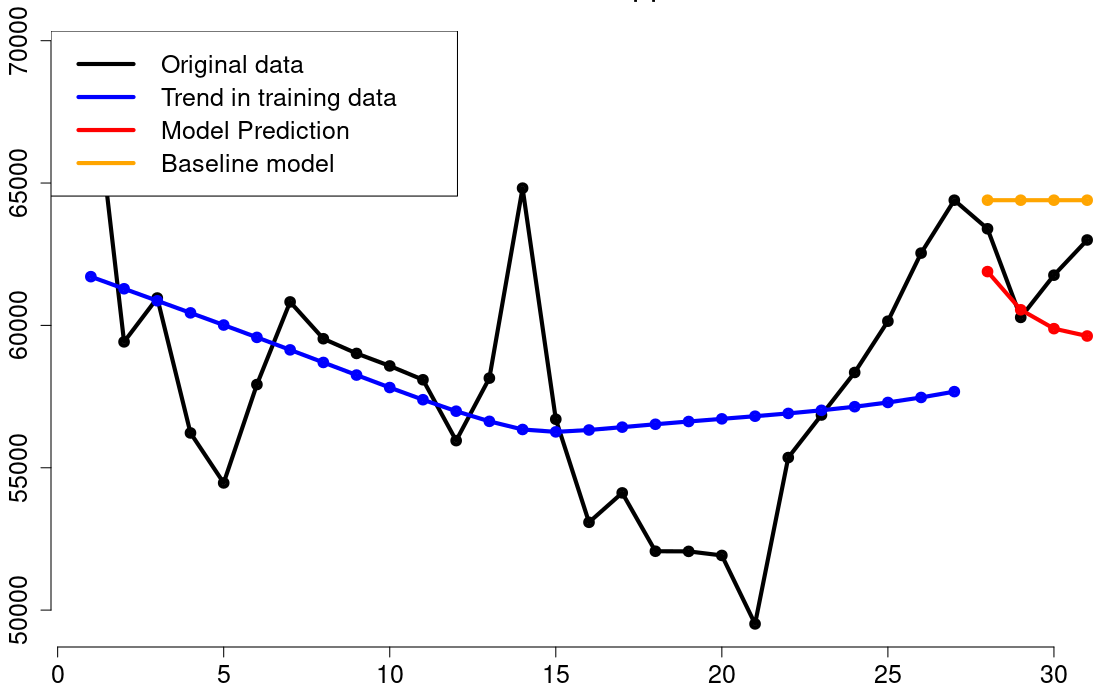
\includegraphics[width=0.8\textwidth]{image1.png}
		\caption{A prediction of four months into the future using the $\mathtt{LOESS}$+$\mathtt{ARMA}(p,q)$-model. Here, the model successfully picked up on the decreasing price in the first two predicted months. The baseline model is added for comparison.}
		\label{fig:image1}
	\end{figure}
	
	\section*{Conclusion}
	Due to the high volatility of the data, predicting the SMEB price one month into the future is difficult and the best results are obtained by simply predicting the previous month's SMEB price. This outperforms all other models which we have tried to fit to the data. For predicting multiple months into the future, certain time series models are able to pick up on the trend of the price and outperform the baseline model.
	
	\section*{Future Recommendations}
	We suggest to look up external events which could explain the sudden peaks and otherwise seemly random volatility of the SMEB price. Including such features into the model could significantly improve the predictive performance.
	
	\section*{Code}
	Aside from the data-cleaning script which we have used, we provide the script which performs the experiment described in Figure~\ref{fig:image2}. Furthermore, we have added the code to evaluate the predictive power of the $\mathtt{LOESS}$+$\mathtt{ARMA}(p,q)$ model as well as a function which allows to make custom predictions with this model. We refer to the README-files for more information on how to run the code. A note on the data which we use: The current implementation of the code uses a file which was given to us by the Hack4Good imputation team. Details regarding this file can be found in the README files.
	
	\section*{Acknowledgments}
	We want to thank the Hack4Good organizational team and IMPACT Initiatives for their efforts and for making this project possible. Furthermore, we want to thank our mentor Anastasia Pentina from the Swiss Data Science Center for her help and advise regarding our project.
\end{document}